\documentclass[a4paper,10pt]{article}
\usepackage[a4paper,left=15mm,right=15mm,top=20mm,bottom=20mm]{geometry}  % 設置頁面的環境, a4紙張大小,左右上邊距信息
\usepackage{indentfirst}  %用首行縮排要引入這個
\usepackage{physics}  %用 braket 用引入這個
%\usepackage{amsmath}  %用矩陣用引入這個
\usepackage{graphicx}  %插入圖片用這個
\usepackage{mathtools}
\usepackage{cancel}
\usepackage{bm}
\allowdisplaybreaks[4]
 \setlength{\parindent}{2em}

\title{Computational Astrophysic\\Homework 2}
\author{d07222009 Guan-Ming Su}
\date{\today}       %日期

\begin{document}

\maketitle

%标题开始
\section*{Problem 1}
 \setlength{\parindent}{0em}(a)
In this problem, we simulated the strong shock Riemann problem using Lax-Friedrichs, Lax-Wendroff, MUSCL-Hancock schemes, and GAMER, compared with the analytical solution. The simulated density $rho$, velocity $v_x$ and pressure $P$ are plotted in Fig. 1, 2, and 3. It is obvious that Lax-Friedrichs scheme is unable to depict the sharp transition between different wave region, due to the strong dissipation. Lax-Wendroff solved the dissipation problem; however, it introduces artifical high-k wave around the transition region. As for the MUSCL-Hancock scheme, we can see that it catches the shock wave quite successfully: density, velocity and pressure are all close to the analytical result. Nevertheless, the GAMER seems to out-perform MUSCL-Hancock: it consumes fewer points to resolve the shock wave front and the contact discontinuity, as shown in the zoom-in figures for each physical quanties around the contact discontinuity or shock region. This might due to its capability of changing gridding adaptively (For Lax-Wendroff, MUSCL-Hancock schemes, and GAMER, the simulated curves along with the analytical counter-parts are shifted for clearness).
%插入圖片
\begin{figure}[htbp] %htbp 代表图片插入位置的设置
\centering %圖片置中
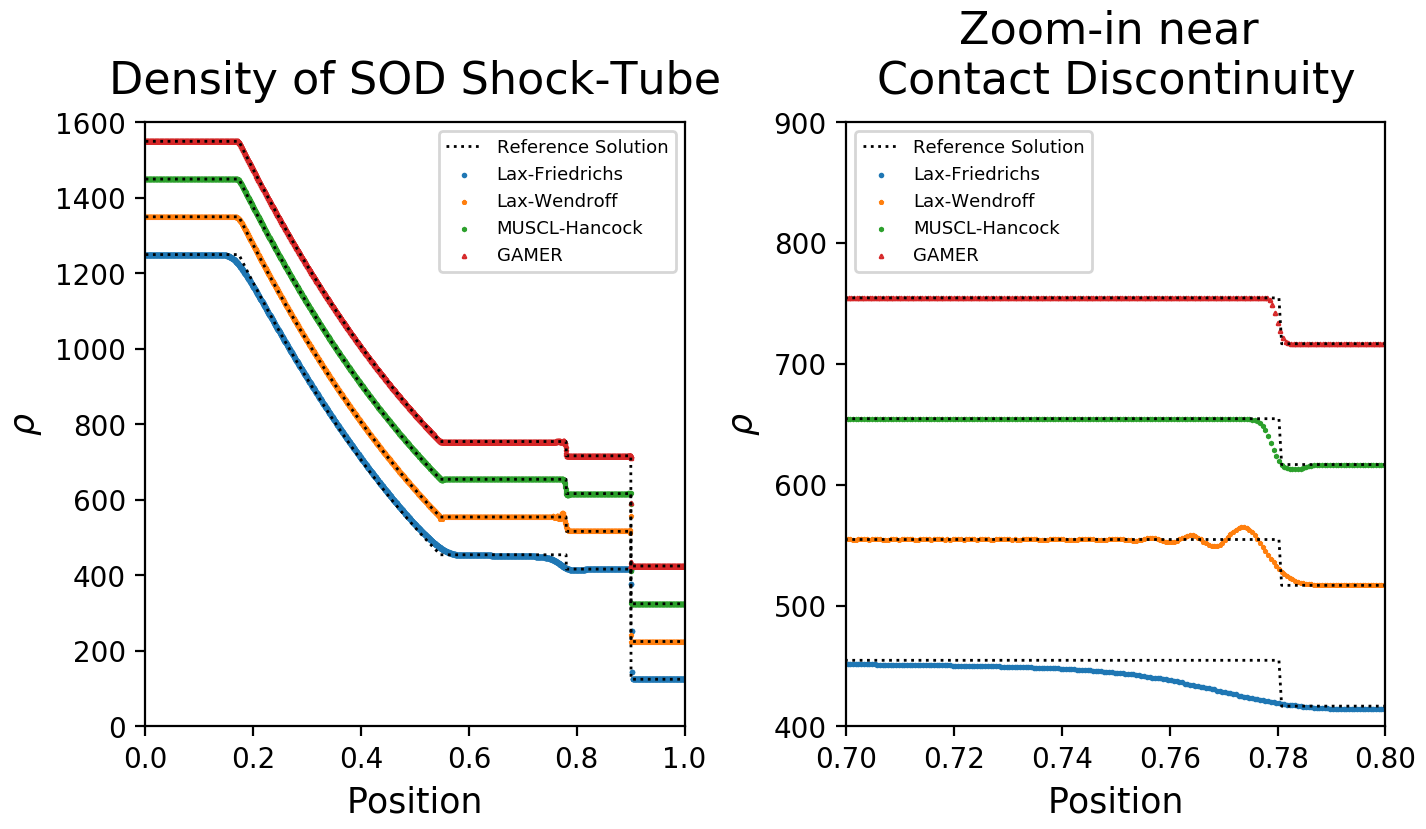
\includegraphics[width=15cm]{density_1-1.png} %[]可選參數,控制圖片大小
%圖片說明
\caption{Density of Strong Shock}
\end{figure}

\begin{figure}[htbp] %htbp 代表图片插入位置的设置
\centering %圖片置中
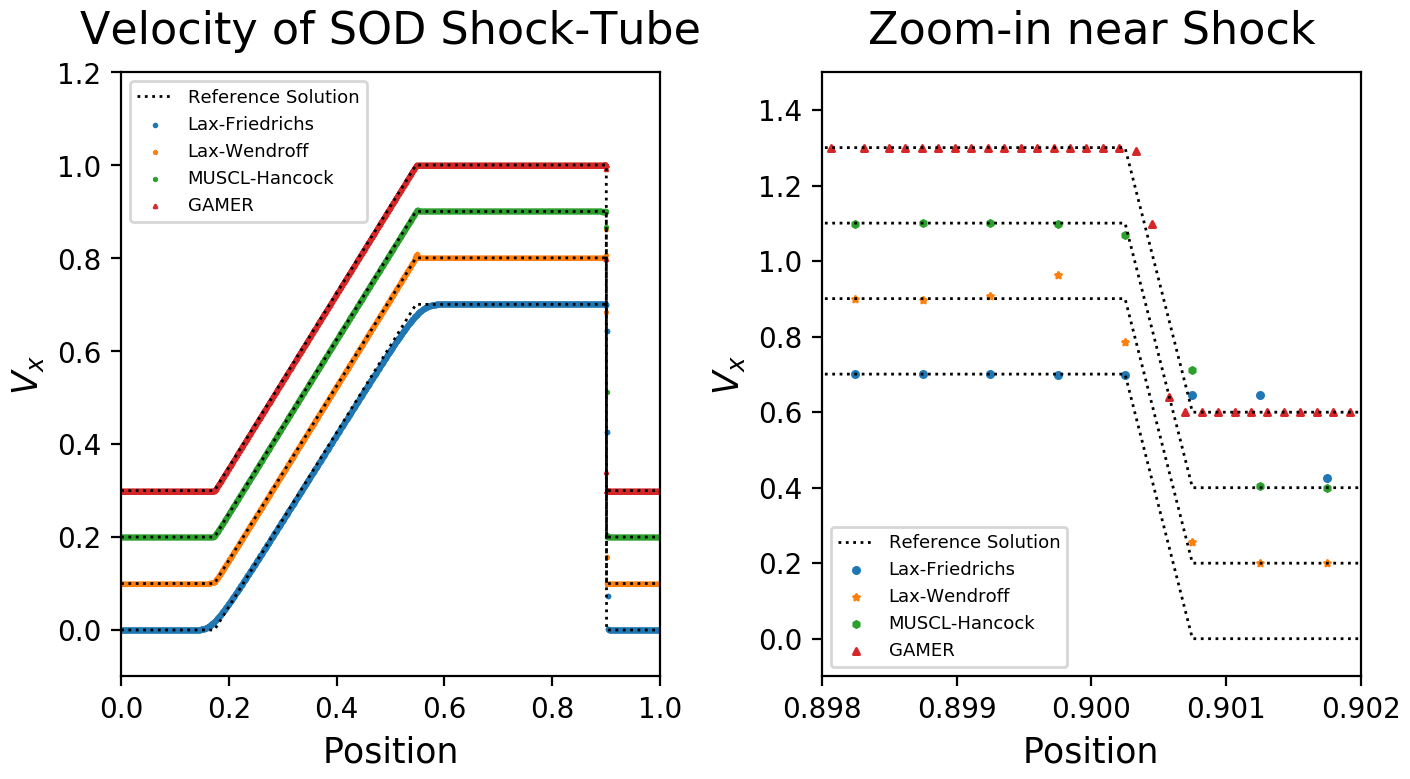
\includegraphics[width=15cm]{velocity_1-1.png} %[]可選參數,控制圖片大小
%圖片說明
\caption{Velocity of Strong Shock}
\end{figure}

\begin{figure}[htbp] %htbp 代表图片插入位置的设置
\centering %圖片置中
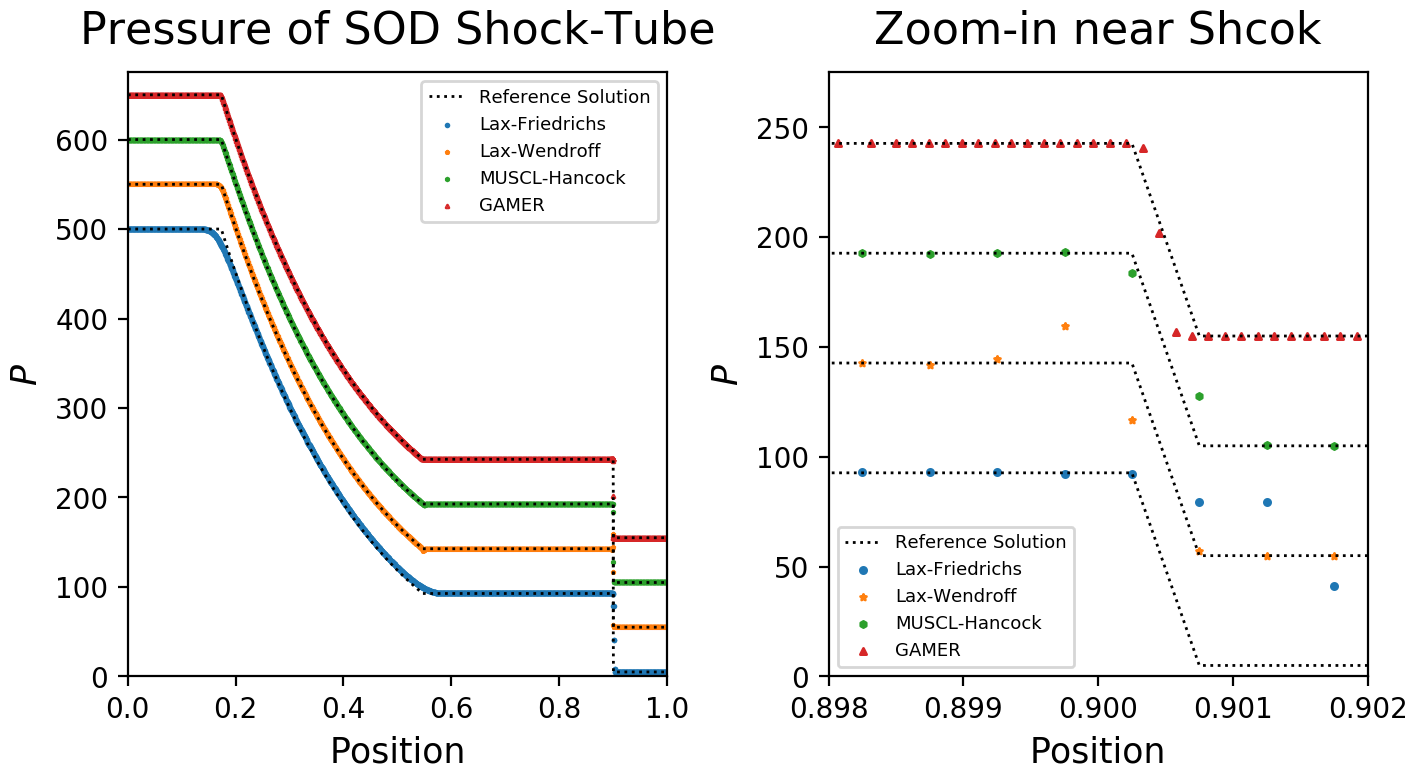
\includegraphics[width=15cm]{pressure_1-1.png} %[]可選參數,控制圖片大小
%圖片說明
\caption{Pressure of Strong Shock}
\end{figure}
\newpage
\setlength{\parindent}{0em}(b)
In this problem, we tried to crash the MUSCL-Hancock scheme by using initial condition with large velocity, i.e., large kinetic energy, compared with the pressure. The code is "successfully" crashed when inital primitive quanties $\begin{bmatrix*}\rho_L\\V_{xL}\\P_L\end{bmatrix*}=\begin{bmatrix*}[c]0.2\\50.0\\10.0 \end{bmatrix*}$ and $\begin{bmatrix*}\rho_L\\V_{xL}\\P_L\end{bmatrix*}=\begin{bmatrix*}[c]0.125\\-25.0\\1.0\end{bmatrix*}$ are given, from $t=0$ to $t=0.05$. Error of negative pressure popped out soon after only a few updates, which might be caused by the relatively large kinetic energy compared with the internal energy, as mentioned above (We also tried $\begin{bmatrix*}\rho_L\\V_{xL}\\P_L\end{bmatrix*}=\begin{bmatrix*}[c]0.2\\50.0\\50.0 \end{bmatrix*}$ and $\begin{bmatrix*}\rho_R\\V_{xR}\\P_R\end{bmatrix*}=\begin{bmatrix*}[c]0.125\\-25.0\\10.0\end{bmatrix*}$, which did converge). Using dual energy probably can deal with this, however, we found that GAMER is not hampered by this issue as well. GAMER with dual energy scheme is also tried, which does not make much difference, suggesting that adaptive changed gridding itself is enough to tackle the problem caused by overwhelming kinetic energy.. GAMER with density refinement criteria is tested as well, with criteria shown in the table below (For GAMER with dual energy and with refinement criteria, the simulated value are shifted for clearness). 

\begin{table}[h]  %table 里面也可以嵌套tabular,只有tabular是不能加标题的
\centering  %表格居中
\begin{tabular}[t]{|c|c|c|c|c|c|c|}
\hline
Level & 0 & 1 & 2 & 3 &4 &5 \\
\hline
Density  & 0.2 & 0.3 & 0.4 & 0.6 & 0.8 & 1.0 \\
\hline
\end{tabular}
\caption{Refinement Criteria for Riemann Problem (Input\underline{\ }Flag\underline{\ }Rho)}  %表格标题
\end{table}

\begin{figure}[htbp] %htbp 代表图片插入位置的设置
\centering %圖片置中
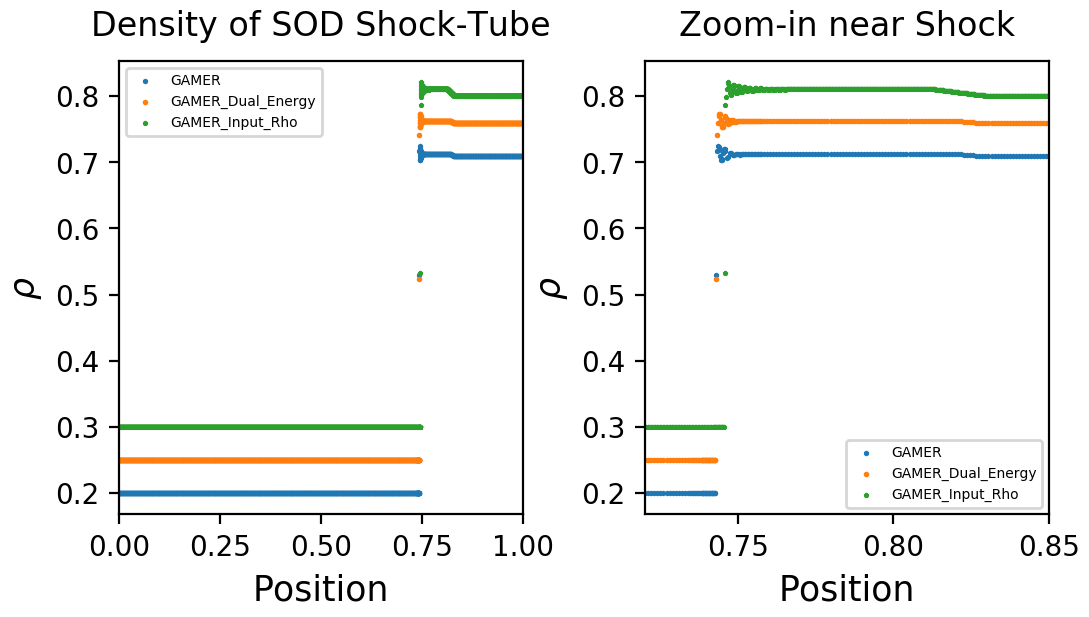
\includegraphics[width=15cm]{density_1-2.png} %[]可選參數,控制圖片大小
%圖片說明
\caption{Density of Riemann Problem with Large Kinetic Energy}
\end{figure}

\begin{figure}[htbp] %htbp 代表图片插入位置的设置
\centering %圖片置中
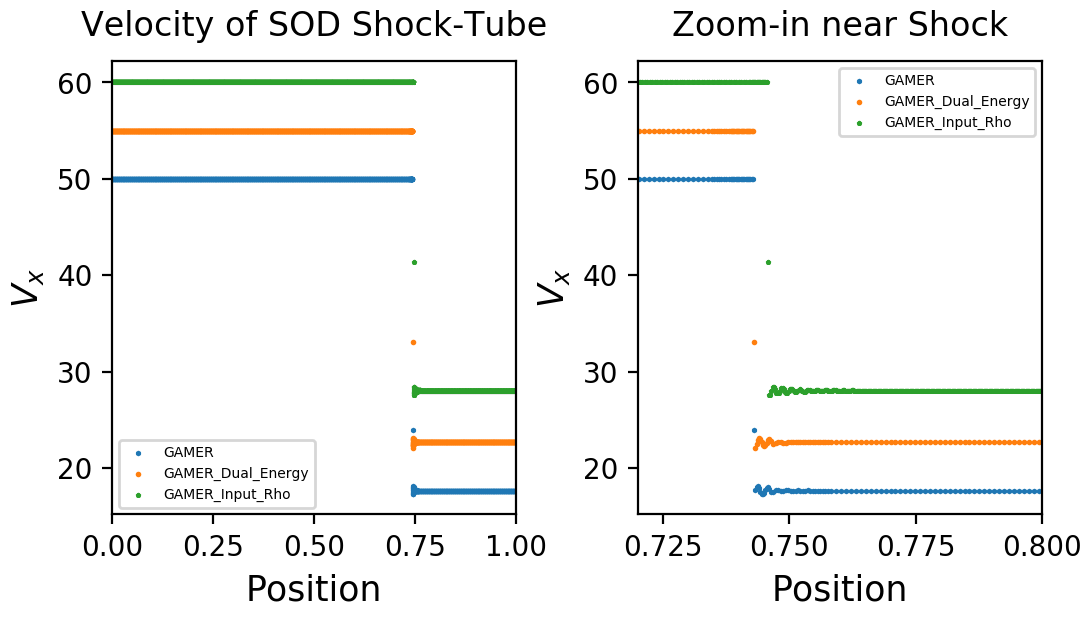
\includegraphics[width=15cm]{velocity_1-2.png} %[]可選參數,控制圖片大小
%圖片說明
\caption{Velocity of Riemann Problem with Large Kinetic Energy}
\end{figure}

\begin{figure}[htbp] %htbp 代表图片插入位置的设置
\centering %圖片置中
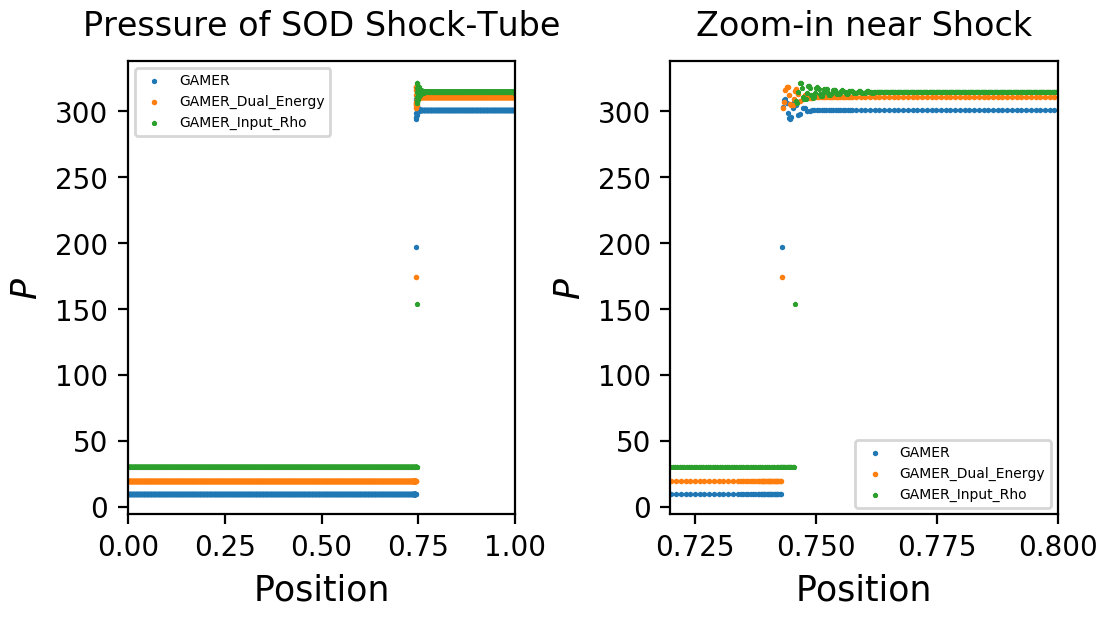
\includegraphics[width=15cm]{pressure_1-2.png} %[]可選參數,控制圖片大小
%圖片說明
\caption{Pressure of Riemann Problem with Large Kinetic Energy}
\end{figure}
\newpage
\section*{Problem 2}
\setlength{\parindent}{0em}(a) Choosen AMR code: GAMER (GPU-accelerated Adaptive Mesh Refinement Code for Astrophysics)

\setlength{\parindent}{0em}(b) The Ryu and Jones Riemann problem (RJ2a), which is similar to Riemann problem but with fluid subjected to magnetic field, is selected as the GAMER test function for the following two reasons: (1) Since the magnetic field is considered here, the problem becomes more complicate with total 8 field components need to be solved. It is interesting to see how well GAMER can do.  (2) A reference solution is provided in the GAMER's example archive, which can be used to validate the simulation result. This 3D problem is gridded in 16x16x16 base-level cells in $x,\ y,\ z$ direction, with refinement criteria specified in Input\underline{\ \ }Flag\underline{\ \ }Rho. The initial condition is given as: $\begin{bmatrix*}\rho_L\\V_{xL}\\V_{yL}\\V_{zL}\\P_L\end{bmatrix*}=\begin{bmatrix*}1.08\\1.2\\0.01\\0.5\\0.95\end{bmatrix*}$; $\begin{bmatrix*}\rho_R\\V_{xR}\\V_{yR}\\V_{zR}\\P_R\end{bmatrix*}=\begin{bmatrix*}1.0\\0.0\\0.0\\0.0\\1.0\end{bmatrix*}$ and  $\begin{bmatrix*}M_{xL}\\M_{yL}\\M_{zL}\end{bmatrix*}=\begin{bmatrix*}\frac{2}{\sqrt{4\pi}}\\\frac{3.6}{\sqrt{4\pi}}\\\frac{2}{\sqrt{4\pi}}\end{bmatrix*}$; $\begin{bmatrix*}M_{xR}\\M_{yR}\\M_{zR}\end{bmatrix*}=\begin{bmatrix*}\frac{2}{\sqrt{4\pi}}\\\frac{4}{\sqrt{4\pi}}\\\frac{2}{\sqrt{4\pi}}\end{bmatrix*}$. Time evolves from 0 to 0.2 .\\
 \setlength{\parindent}{0em}(c) The refinement criteria is specified in the Input\underline{\ }Flat\underline{\ }Rho, where the content is listed below:

\begin{table}[h]  %table 里面也可以嵌套tabular,只有tabular是不能加标题的
\centering  %表格居中
\begin{tabular}[t]{|c|c|c|c|c|c|c|}
\hline
Level & 0 & 1 & 2 & 3 &4 &5 \\
\hline
Density  & 1.0 & 1.1 & 1.2 & 1.3 & 1.4 & 1.45 \\
\hline
\end{tabular}
\caption{Refinement Criteria for RJ2a (Input\underline{\ }Flag\underline{\ }Rho)}  %表格标题
\end{table}

While the compile parameter -DNLEVEL is set as 10 in the Makefile, we constrainted the available level by runtime parameter MAX\underline{\ }LEVEL, varying from 0 to 5, which affects the result quite significantly (shall be shown in (f)). Another criteria is set in the Input\underline{\ }Flag\underline{\ }Lohner, as listed below

\begin{table}[h]  %table 里面也可以嵌套tabular,只有tabular是不能加标题的
\centering  %表格居中
\begin{tabular}[t]{|c|c|c|c|c|}
\hline
Level & Threshold & Filter & Soften & MinDensity\\
\hline
0  & 0.50 & 0.01 & 0.00 & 0.00\\
\hline
1  & 0.50 & 0.01 & 0.00 & 0.00\\
\hline
2  & 0.50 & 0.01 & 0.00 & 0.00\\
\hline
3  & 0.50 & 0.01 & 0.00 & 0.00\\
\hline
4  & 0.50 & 0.01 & 0.00 & 0.00\\
\hline
5  & 0.50 & 0.01 & 0.00 & 0.00\\
\hline
6  & 0.50 & 0.01 & 0.00 & 0.00\\
\hline
7  & 0.50 & 0.01 & 0.00 & 0.00\\
\hline
8  & 0.50 & 0.01 & 0.00 & 0.00\\
\hline
9  & 0.50 & 0.01 & 0.00 & 0.00\\
\hline
10  & 0.50 & 0.01 & 0.00 & 0.00\\
\hline
11  & 0.50 & 0.01 & 0.00 & 0.00\\
\hline
\end{tabular}
\caption{Refinement Criteria for RJ2a (Input\underline{\ }Flag\underline{\ }Lohner)}  %表格标题
\end{table}

\setlength{\parindent}{0em}(d) The boundary condition is specified in the Input\underline{\quad}Parameter, where the fluid boundary conditions in $x,\ y, \ z$ are all set to outflow.\\

\setlength{\parindent}{0em}(e) and (f) The result for density $\rho$, pressue $P$, velocity $(V_x, V_y, V_z)$ and  magnetic field $(B_x, B_y, B_z)$ are listed below, with MAX\underline{\ }LEVEL increasing from 0 to 5. Though all simulation converges, we can clearly see that when the AMRlevel increases, the data points overlap more well with the reference curve. The best performance is given by MAX\underline{\ }LEVEL=4 and 5, whose simulation on $\rho$, $P$, $(V_x, V_y, V_z)$ and $(B_x, B_y)$ are quite close to the reference solution; however, the simulated $B_z$ seems to deviates a little bit, especially around $x=0.7$ to $0.9$ region. The time consumed for each simulation with different MAX\underline{\ }LEVEL is also attached.

\begin{table}[h]  %table 里面也可以嵌套tabular,只有tabular是不能加标题的
\centering  %表格居中
\begin{tabular}[t]{|c|c|c|c|c|c|c|}
\hline
MAX\underline{\ }LEVEL & 0 & 1 & 2 & 3 &4 &5 \\
\hline
Time(s)  & 0.393366 & 0.606961 & 2.486324  & 23.490036 & 197.151280 & 2038.830045 \\
\hline
\end{tabular}
\caption{Time Consumed by RJ2a with Different MAX\underline{\ }LEVEL}  %表格标题
\end{table}

\begin{figure}[htbp] %htbp 代表图片插入位置的设置
\centering %圖片置中
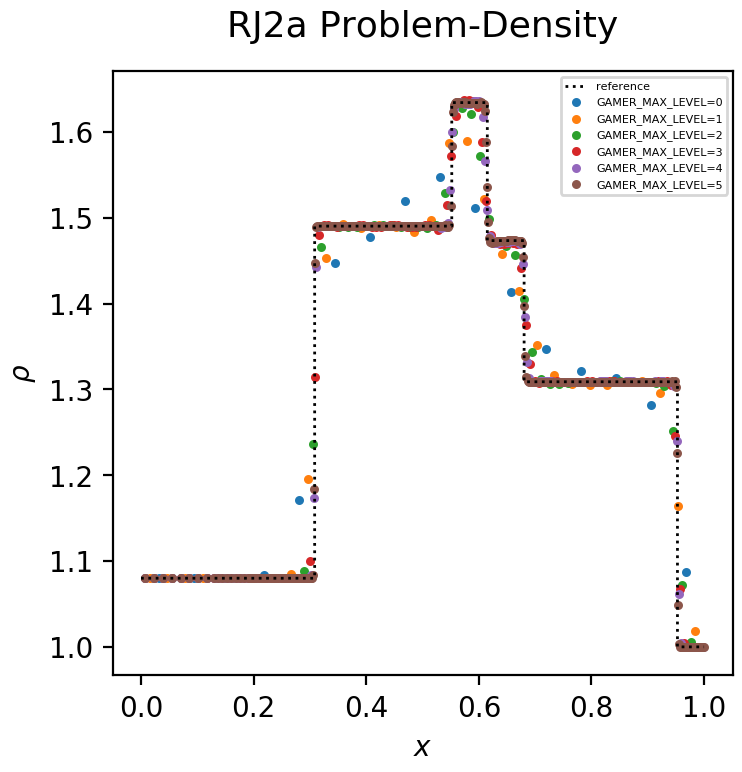
\includegraphics[width=10cm]{density_2.png} %[]可選參數,控制圖片大小
%圖片說明
\caption{Density of RJ2a Problem}
\end{figure}

\begin{figure}[htbp] %htbp 代表图片插入位置的设置
\centering %圖片置中
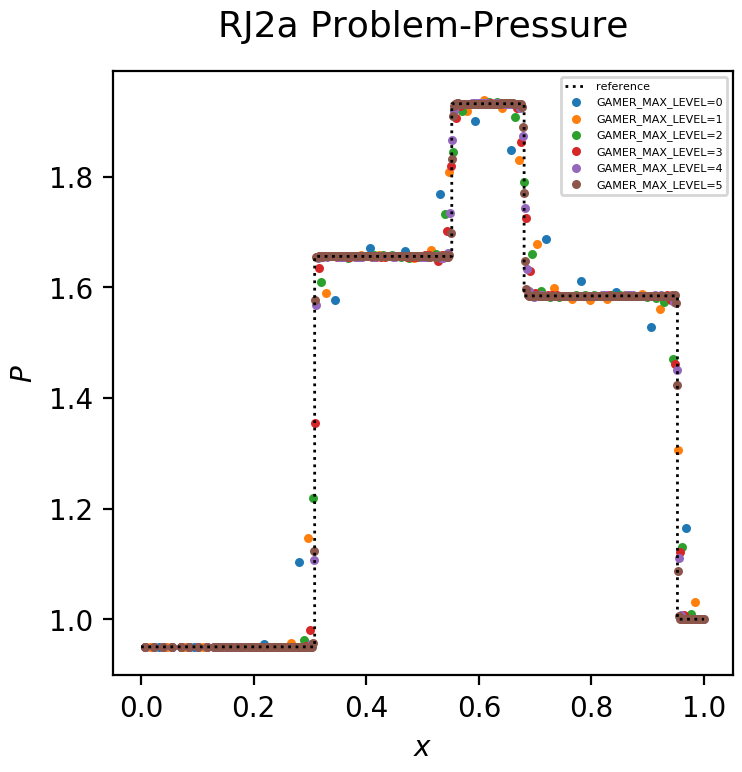
\includegraphics[width=10cm]{pressure_2.png} %[]可選參數,控制圖片大小
%圖片說明
\caption{Pressure of RJ2a Problem}
\end{figure}

\begin{figure}[htbp] %htbp 代表图片插入位置的设置
\centering %圖片置中
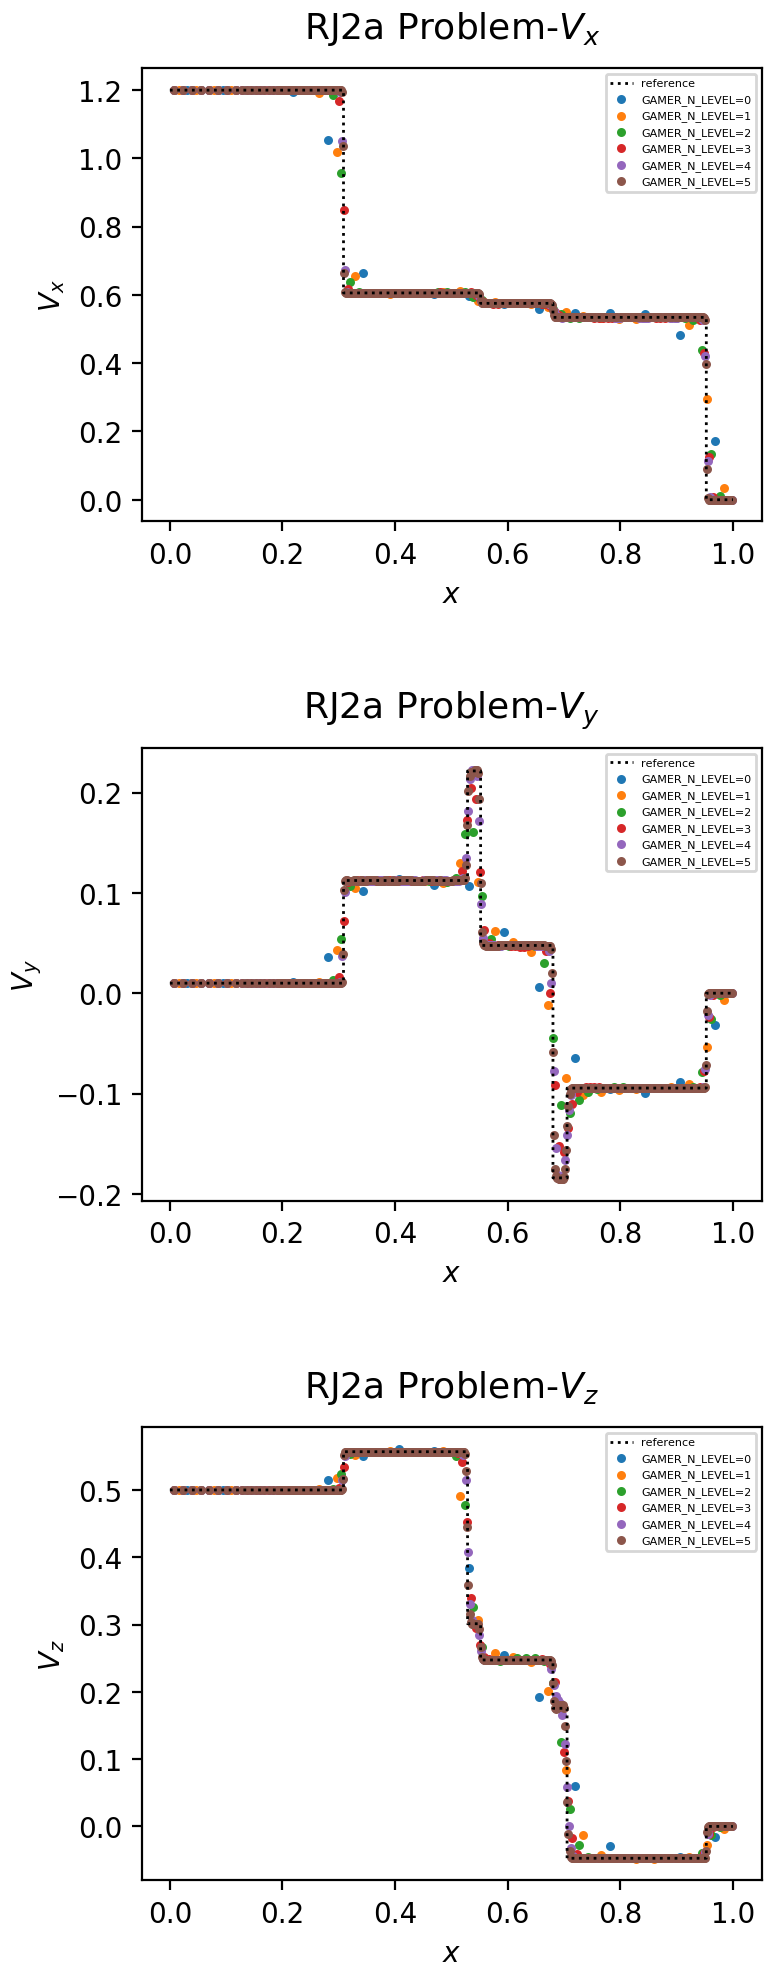
\includegraphics[width=8cm]{velocity_2.png} %[]可選參數,控制圖片大小
%圖片說明
\caption{Velocity of RJ2a Problem}
\end{figure}

\begin{figure}[htbp] %htbp 代表图片插入位置的设置
\centering %圖片置中
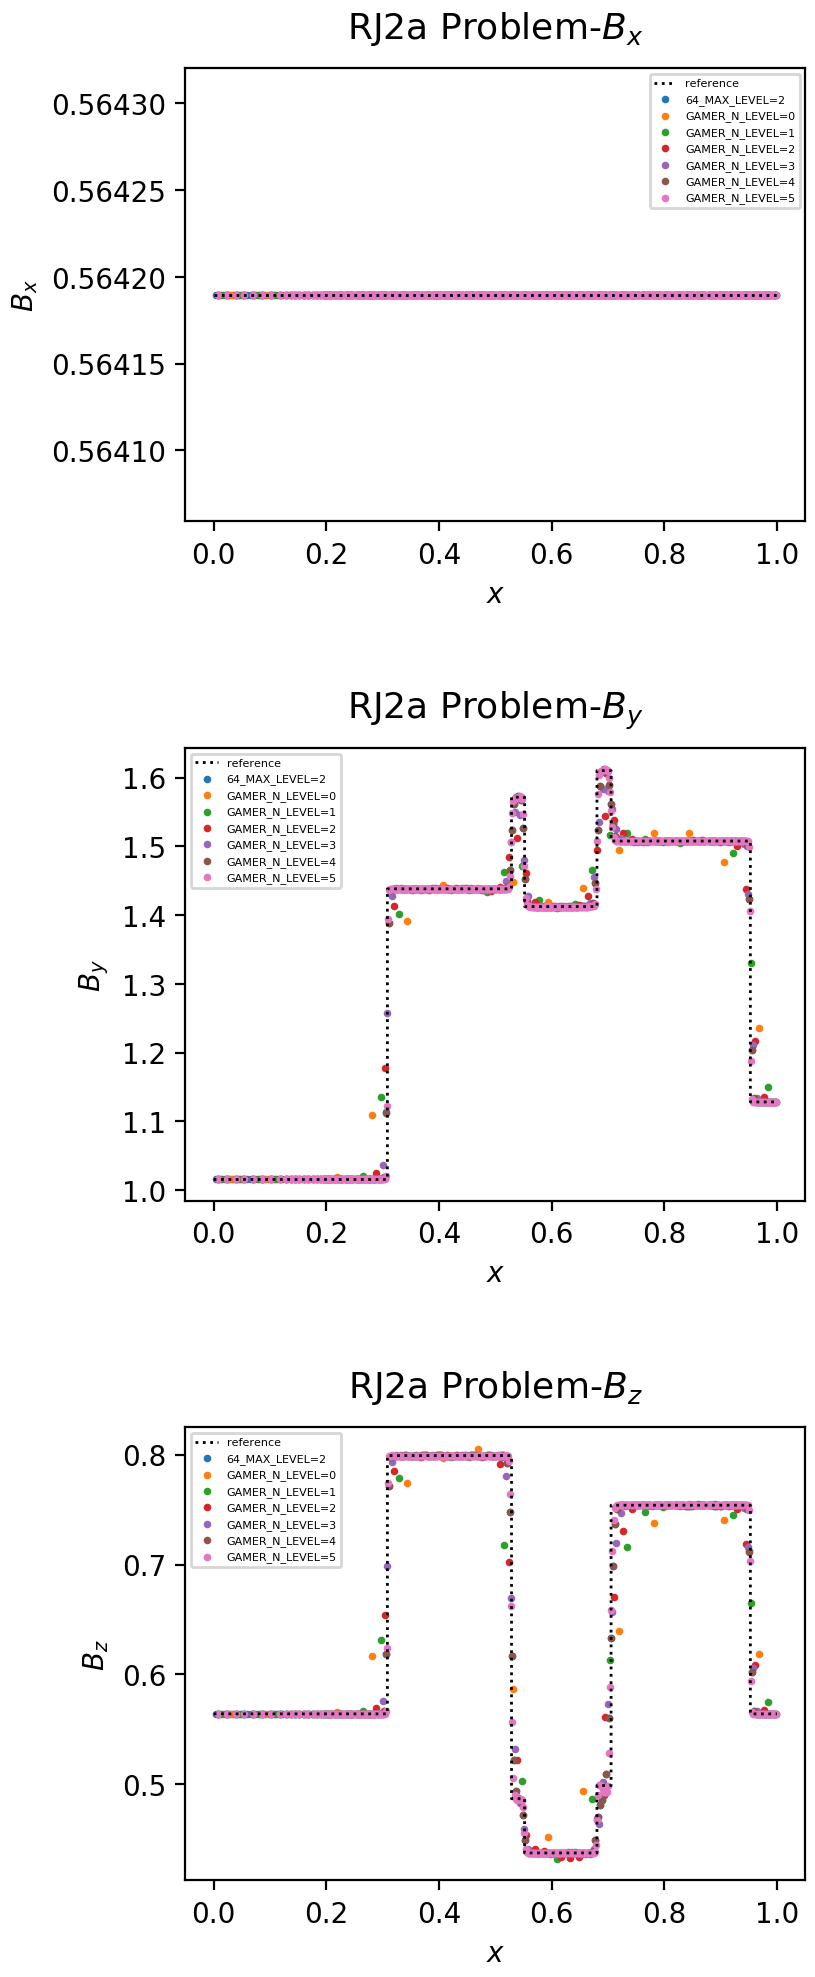
\includegraphics[width=8cm]{field_2.png} %[]可選參數,控制圖片大小
%圖片說明
\caption{Magnetic Field of RJ2a Problem}
\end{figure}

\newpage
\section*{Problem 3}
{\parindent0pt % disables indentation for all the text between { and }
\textbf{Demonstrate that the CT(Constrainted Transport) update guarantees \\ \bm{$\nabla\cdot B^{n+1}=\nabla \cdot B^n}$ in 3D.}}

From the relation between area-averaged magnetic field and time-and-line-averaged EMF:
\begin{align}
\begin{cases}
B_{x,i\pm\frac{1}{2},j,k}^{n+1}-B_{x,i\pm\frac{1}{2},j,k}^{n}=-\frac{\Delta t}{\Delta z}(\epsilon_{y,i\pm\frac{1}{2},j,k-\frac{1}{2}}^{n+\frac{1}{2}}-\epsilon_{y,i\pm\frac{1}{2},j,k+\frac{1}{2}}^{n+\frac{1}{2}})-\frac{\Delta t}{\Delta y}(\epsilon_{z,i\pm\frac{1}{2},j+\frac{1}{2},k}^{n+\frac{1}{2}}-\epsilon_{z,i\pm\frac{1}{2},j-\frac{1}{2},k}^{n+\frac{1}{2}}) \\
B_{y,i,j\pm\frac{1}{2},k}^{n+1}-B_{y,i,j\pm\frac{1}{2},k}^{n}=-\frac{\Delta t}{\Delta x}(\epsilon_{z,i-\frac{1}{2},j\pm\frac{1}{2},k}^{n+\frac{1}{2}}-\epsilon_{z,i+\frac{1}{2},j\pm\frac{1}{2},k}^{n+\frac{1}{2}})-\frac{\Delta t}{\Delta z}(\epsilon_{x,i,j\pm\frac{1}{2},k+\frac{1}{2}}^{n+\frac{1}{2}}-\epsilon_{x,i,j\pm\frac{1}{2},k-\frac{1}{2}}^{n+\frac{1}{2}}) \\
B_{z,i,j,k\pm\frac{1}{2}}^{n+1}-B_{z,i,j,k\pm\frac{1}{2}}^{n}=-\frac{\Delta t}{\Delta y}(\epsilon_{x,i,j-\frac{1}{2},k\pm\frac{1}{2}}^{n+\frac{1}{2}}-\epsilon_{x,i,j+\frac{1}{2},k\pm\frac{1}{2}}^{n+\frac{1}{2}})-\frac{\Delta t}{\Delta x}(\epsilon_{y,i+\frac{1}{2},j,k\pm\frac{1}{2}}^{n+\frac{1}{2}}-\epsilon_{y,i-\frac{1}{2},j,k\pm\frac{1}{2}}^{n+\frac{1}{2}})\\
\end{cases}
\end{align}
along with the discretized form of:
\begin{align}
\nabla \cdot B \Rightarrow\frac{1}{\Delta x}(B_{x,i+\frac{1}{2},j,k}^n-B_{x,i-\frac{1}{2},j,k}^n)+\frac{1}{\Delta y}(B_{y,i,j+\frac{1}{2},k}^n-B_{x,i,j-\frac{1}{2},k}^n)+\frac{1}{z}(B_{z,i,j,k+\frac{1}{2}}^n-B_{z,i,j,k-\frac{1}{2}}^n)
\end{align}
we have:
\begin{align}
\nabla \cdot B^{n+1}-\nabla \cdot B^{n}
=&\frac{1}{\Delta x}(B_{x,i+\frac{1}{2},j,k}^{n+1}-B_{x,i+\frac{1}{2},j,k}^n-B_{x,i-\frac{1}{2},j,k}^{n+1}+B_{x,i-\frac{1}{2},j,k}^n) \notag \\
+&\frac{1}{\Delta y}(B_{y,i,j+\frac{1}{2},k}^{n+1}-B_{y,i,j+\frac{1}{2},k}^n-B_{y,i,j-\frac{1}{2},k}^{n+1}+B_{y,i,j-\frac{1}{2},k}^n) \notag \\
+&\frac{1}{\Delta z}(B_{z,i,j,k+\frac{1}{2}}^{n+1}-B_{z,i,j,k+\frac{1}{2}}^n-B_{z,i,j,k-\frac{1}{2}}^{n+1}+B_{z,i,j,k-\frac{1}{2}}^n) \notag \\
=&-\frac{\Delta t}{\Delta x}(\frac{1}{\Delta z}(\epsilon_{y,i+\frac{1}{2},j,k-\frac{1}{2}}^{n+\frac{1}{2}}-\epsilon_{y,i+\frac{1}{2},j,k+\frac{1}{2}}^{n+\frac{1}{2}})+\frac{1}{\Delta y}(\epsilon_{z,i+\frac{1}{2},j+\frac{1}{2},k}^{n+\frac{1}{2}}-\epsilon_{z,i+\frac{1}{2},j-\frac{1}{2},k}^{n+\frac{1}{2}}) \notag \\
&\quad\quad-\frac{1}{\Delta z}(\epsilon_{y,i-\frac{1}{2},j,k-\frac{1}{2}}^{n+\frac{1}{2}}-\epsilon_{y,i-\frac{1}{2},j,k+\frac{1}{2}}^{n+\frac{1}{2}})-\frac{1}{\Delta y}(\epsilon_{z,i-\frac{1}{2},j+\frac{1}{2},k}^{n+\frac{1}{2}}-\epsilon_{z,i-\frac{1}{2},j-\frac{1}{2},k}^{n+\frac{1}{2}})) \notag \\
&-\frac{\Delta t}{\Delta y}(\frac{1}{\Delta x}(\epsilon_{z,i-\frac{1}{2},j+\frac{1}{2},k}^{n+\frac{1}{2}}-\epsilon_{z,i+\frac{1}{2},j+\frac{1}{2},k}^{n+\frac{1}{2}})+\frac{1}{\Delta z}(\epsilon_{x,i,j+\frac{1}{2},k+\frac{1}{2}}^{n+\frac{1}{2}}-\epsilon_{x,i,j+\frac{1}{2},k-\frac{1}{2}}^{n+\frac{1}{2}}) \notag \\
&\quad\quad-\frac{1}{\Delta x}(\epsilon_{z,i-\frac{1}{2},j-\frac{1}{2},k}^{n+\frac{1}{2}}-\epsilon_{z,i+\frac{1}{2},j-\frac{1}{2},k}^{n+\frac{1}{2}})-\frac{1}{\Delta z}(\epsilon_{x,i,j-\frac{1}{2},k+\frac{1}{2}}^{n+\frac{1}{2}}-\epsilon_{x,i,j-\frac{1}{2},k-\frac{1}{2}}^{n+\frac{1}{2}})) \notag \\
&-\frac{\Delta t}{\Delta z}(\frac{1}{\Delta y}(\epsilon_{x,i,j-\frac{1}{2},k+\frac{1}{2}}^{n+\frac{1}{2}}-\epsilon_{x,i,j+\frac{1}{2},k+\frac{1}{2}}^{n+\frac{1}{2}})+\frac{1}{\Delta x}(\epsilon_{y,i+\frac{1}{2},j,k+\frac{1}{2}}^{n+\frac{1}{2}}-\epsilon_{y,i-\frac{1}{2},j,k+\frac{1}{2}}^{n+\frac{1}{2}}) \notag \\
&\quad\quad-\frac{1}{\Delta y}(\epsilon_{x,i,j-\frac{1}{2},k-\frac{1}{2}}^{n+\frac{1}{2}}-\epsilon_{x,i,j+\frac{1}{2},k-\frac{1}{2}}^{n+\frac{1}{2}})-\frac{1}{\Delta x}(\epsilon_{y,i+\frac{1}{2},j,k-\frac{1}{2}}^{n+\frac{1}{2}}-\epsilon_{y,i-\frac{1}{2},j,k-\frac{1}{2}}^{n+\frac{1}{2}})) \notag \\
=&-\frac{\Delta t}{\Delta z\Delta x}(\bcancel{\epsilon_{y,i+\frac{1}{2},j,k-\frac{1}{2}}^{n+\frac{1}{2}}}-\bcancel{\epsilon_{y,i+\frac{1}{2},j,k+\frac{1}{2}}^{n+\frac{1}{2}}}-\bcancel{\epsilon_{y,i-\frac{1}{2},j,k-\frac{1}{2}}^{n+\frac{1}{2}}}+\bcancel{\epsilon_{y,i-\frac{1}{2},j,k+\frac{1}{2}}^{n+\frac{1}{2}}} \notag \\
&\quad\quad\quad\ +\bcancel{\epsilon_{y,i+\frac{1}{2},j,k+\frac{1}{2}}^{n+\frac{1}{2}}}-\bcancel{\epsilon_{y,i-\frac{1}{2},j,k+\frac{1}{2}}^{n+\frac{1}{2}}}-\bcancel{\epsilon_{y,i+\frac{1}{2},j,k-\frac{1}{2}}^{n+\frac{1}{2}}}+\bcancel{\epsilon_{y,i-\frac{1}{2},j,k-\frac{1}{2}}^{n+\frac{1}{2}}}) \notag \\
&-\frac{\Delta t}{\Delta x\Delta y}(\bcancel{\epsilon_{z,i+\frac{1}{2},j+\frac{1}{2},k}^{n+\frac{1}{2}}}-\bcancel{\epsilon_{z,i+\frac{1}{2},j-\frac{1}{2},k}^{n+\frac{1}{2}}}-\bcancel{\epsilon_{z,i-\frac{1}{2},j+\frac{1}{2},k}^{n+\frac{1}{2}}}+\bcancel{\epsilon_{z,i-\frac{1}{2},j-\frac{1}{2},k}^{n+\frac{1}{2}}} \notag \\
&\quad\quad\quad\ +\bcancel{\epsilon_{z,i-\frac{1}{2},j+\frac{1}{2},k}^{n+\frac{1}{2}}}-\bcancel{\epsilon_{z,i+\frac{1}{2},j+\frac{1}{2},k}^{n+\frac{1}{2}}}-\bcancel{\epsilon_{z,i-\frac{1}{2},j-\frac{1}{2},k}^{n+\frac{1}{2}}}+\bcancel{\epsilon_{z,i+\frac{1}{2},j-\frac{1}{2},k}^{n+\frac{1}{2}}}) \notag \\
&-\frac{\Delta t}{\Delta y\Delta z}(\bcancel{\epsilon_{x,i,j-\frac{1}{2},k+\frac{1}{2}}^{n+\frac{1}{2}}}-\bcancel{\epsilon_{x,i,j+\frac{1}{2},k+\frac{1}{2}}^{n+\frac{1}{2}}}-\bcancel{\epsilon_{x,i,j-\frac{1}{2},k-\frac{1}{2}}^{n+\frac{1}{2}}}+\bcancel{\epsilon_{x,i,j+\frac{1}{2},k-\frac{1}{2}}^{n+\frac{1}{2}}} \notag \\
&\quad\quad\quad\ +\bcancel{\epsilon_{x,i,j+\frac{1}{2},k+\frac{1}{2}}^{n+\frac{1}{2}}}-\bcancel{\epsilon_{x,i,j+\frac{1}{2},k-\frac{1}{2}}^{n+\frac{1}{2}}}-\bcancel{\epsilon_{x,i,j-\frac{1}{2},k+\frac{1}{2}}^{n+\frac{1}{2}}}+\bcancel{\epsilon_{x,i,j-\frac{1}{2},k-\frac{1}{2}}^{n+\frac{1}{2}}}) \\
=&0 \notag 
\end{align}
which guarantees that $\nabla\cdot B$ is conserved for each updating, but one still need to choose the proper initial condition to realize  $\nabla\cdot B=0$.

\end{document}
